% A filter and a merit-function isovalue on the same axes.
%
%   figures/tikz/cg-filter.tex
%       -> media/figures/cg-filter.{png,svg}
%
% Lecture 22 (Globalization for Constrained Optimization), section VIII "Filters",
% subsection "The acceptance margin". Moved 2026-10-07 from the inline tikzpicture in
% lecture-notes/lectures/constrained-globalization.tex (format pass); the geometry is
% unchanged, only the styling is new.
%
% CONTENT: N&W Fig. 15.7 (merit isovalue over the filter staircase), pp. 438-439, with the
% gamma-margin of Biegler Fig. 5.3, p. 112. Four filter pairs (h, f):
%   (1.0, 4.0), (2.2, 2.9), (3.6, 2.0), (5.2, 1.2).
% The forbidden region is everything up-right of the staircase through them. The dotted
% margin is the staircase shifted by -0.25 in both coordinates, i.e. parallel to it: the
% rectangular envelope (2.5) of Fletcher, Leyffer & Toint (2002), p. 46, which is the shape
% of Biegler's (5.60) (margin taken on the current iterate). Their Fig. 1, p. 47, draws the
% SLANTING envelope (2.6) instead; do not put the two side by side without saying so.
% The merit isovalue f + rho ||h|| = const is the straight line from (1.6, 3.8) to (5.6, 0.2).
%
% GREYSCALE: the forbidden region is HATCHED (not tinted), the staircase is solid, the
% margin is dotted and the merit isovalue is dashed and labelled, so no distinction rests on
% colour. No acceptance verdicts beyond the two region labels are printed: the activity after
% the figure asks for them.
\usetikzlibrary{patterns}
\definecolor{okabeblue}{HTML}{0072B2}
\definecolor{okabever}{HTML}{D55E00}

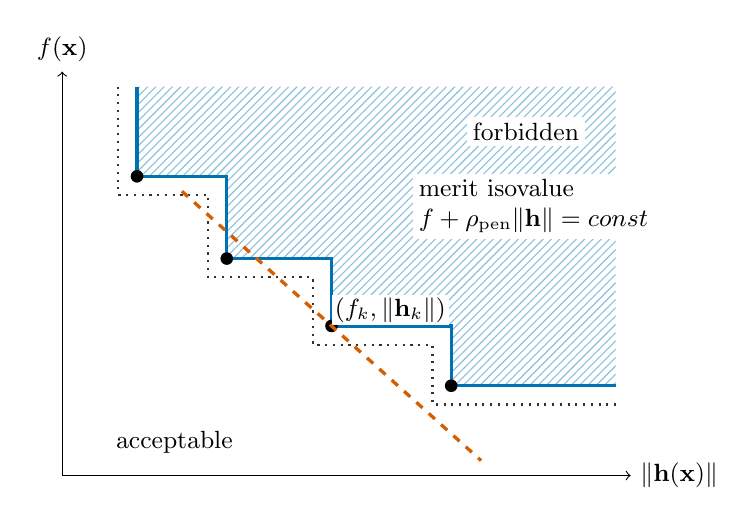
\begin{tikzpicture}[scale=0.95, font=\small]
  % forbidden region (hatched)
  \path[pattern=north east lines, pattern color=okabeblue!45]
    (1.0,5.2) -- (1.0,4.0) -- (2.2,4.0) -- (2.2,2.9)
    -- (3.6,2.9) -- (3.6,2.0) -- (5.2,2.0) -- (5.2,1.2) -- (7.4,1.2)
    -- (7.4,5.2) -- cycle;
  % axes
  \draw[->] (0,0) -- (7.6,0) node[right] {$\|\mathbf{h}(\mathbf{x})\|$};
  \draw[->] (0,0) -- (0,5.4) node[above] {$f(\mathbf{x})$};
  % filter staircase (solid)
  \draw[very thick, okabeblue]
    (1.0,5.2) -- (1.0,4.0) -- (2.2,4.0) -- (2.2,2.9)
    -- (3.6,2.9) -- (3.6,2.0) -- (5.2,2.0) -- (5.2,1.2) -- (7.4,1.2);
  % gamma margin (dotted)
  \draw[dotted, thick, black!80]
    (0.75,5.2) -- (0.75,3.75) -- (1.95,3.75) -- (1.95,2.65)
    -- (3.35,2.65) -- (3.35,1.75) -- (4.95,1.75) -- (4.95,0.95) -- (7.4,0.95);
  % filter pairs
  \fill (1.0,4.0) circle (2.4pt);
  \fill (2.2,2.9) circle (2.4pt);
  \fill (3.6,2.0) circle (2.4pt);
  \fill (5.2,1.2) circle (2.4pt);
  \node[above right, fill=white, inner sep=1pt] at (3.6,2.0) {$(f_k, \|\mathbf{h}_k\|)$};
  % merit function isovalue through the current pair (dashed)
  \draw[very thick, dashed, okabever] (1.6,3.8) -- (5.6,0.2);
  \node[align=left, fill=white, inner sep=2pt] at (6.3,3.6)
    {merit isovalue\\ $f + \rho_{\mathrm{pen}}\|\mathbf{h}\| = \text{const}$};
  \node[fill=white, inner sep=2pt] at (6.2,4.6) {forbidden};
  \node at (1.5,0.45) {acceptable};
\end{tikzpicture}
